% !TEX program = xelatex
\documentclass[12pt,a4paper]{article}

\usepackage[a4paper,margin=2.4cm,headheight=16pt]{geometry}
\usepackage{fontspec}
\usepackage[brazil]{babel}
\usepackage{graphicx}
\usepackage{float}
\usepackage{booktabs}
\usepackage{tabularx}
\usepackage{array}
\usepackage{xcolor}
\usepackage{hyperref}
\usepackage{caption}
\usepackage{subcaption}
\usepackage{enumitem}
\usepackage{titlesec}
\usepackage{fancyhdr}
\usepackage{lastpage}

\setmainfont{TeX Gyre Termes}

\definecolor{utfprblack}{HTML}{1F2933}
\definecolor{utfpryellow}{HTML}{F2B705}
\definecolor{softgray}{HTML}{F3F4F6}
\definecolor{linegray}{HTML}{D6D8DC}

\hypersetup{
    colorlinks=true,
    linkcolor=utfprblack,
    urlcolor=blue
}

\setlength{\parindent}{0pt}
\setlength{\parskip}{6pt}
\setlength{\emergencystretch}{3em}
\sloppy
\renewcommand{\arraystretch}{1.25}

\pagestyle{fancy}
\fancyhf{}
\lhead{\small Jornada da Eletrônica}
\rhead{\small Relatório de Atividade 01}
\cfoot{\small Página \thepage\ de \pageref{LastPage}}
\renewcommand{\headrulewidth}{0.4pt}
\renewcommand{\footrulewidth}{0pt}

\titleformat{\section}
  {\Large\bfseries\color{utfprblack}}
  {\thesection}
  {0.7em}
  {}
  [\vspace{0.2em}{\color{utfpryellow}\titlerule[1.1pt]}]

\titleformat{\subsection}
  {\large\bfseries\color{utfprblack}}
  {\thesubsection}
  {0.6em}
  {}

\captionsetup{
    font=small,
    labelfont=bf,
    justification=centering
}

\newcolumntype{Y}{>{\raggedright\arraybackslash}X}
\newcommand{\email}[1]{\href{mailto:#1}{\nolinkurl{#1}}}

\newcommand{\infobox}[1]{%
    \vspace{0.2cm}
    \noindent
    \colorbox{softgray}{%
        \begin{minipage}{0.96\textwidth}
            \vspace{0.35cm}
            #1
            \vspace{0.35cm}
        \end{minipage}
    }
}

\begin{document}

\begin{titlepage}
    \thispagestyle{empty}
    \begin{center}
        \vspace*{1.2cm}
        {\Large Universidade Tecnológica Federal do Paraná}\\
        {\large Campus Toledo}\\[1.6cm]

        \colorbox{utfpryellow}{%
            \begin{minipage}{0.88\textwidth}
                \centering
                \vspace{0.8cm}
                {\Huge\bfseries Jornada da Eletrônica}\\[0.3cm]
                {\Large Relatório de Atividade 01}\\[0.3cm]
                {\Large Minicurso: Programação do Microcontrolador CH32V003}
                \vspace{0.8cm}
            \end{minipage}
        }\\[1.8cm]

        \begin{tabular}{rl}
            \textbf{Data:} & 22/04/2026 \\
            \textbf{Local:} & Laboratório E207, UTFPR - Campus Toledo \\
            \textbf{Horário:} & 18h40 \\
            \textbf{Ministrante:} & Luis Alberto Martignago \\
            \textbf{Apoio docente:} & Felipe Walter Dafico Pfrimer \\
        \end{tabular}

        \vfill
        Toledo, 2026
    \end{center}
\end{titlepage}

\section{Identificação da Atividade}

\infobox{
\begin{tabularx}{\textwidth}{>{\bfseries}p{0.34\textwidth}Y}
Data & 22/04/2026 \\
Local & Laboratório E207, UTFPR - Campus Toledo \\
Horário & 18h40 \\
Forma de divulgação & Publicação/reels no Instagram do Centro Acadêmico de Engenharia Eletrônica e divulgação em canais de comunicação do curso. \\
Forma de inscrição & Inscrição por QR Code divulgado no material da atividade, com taxa de investimento de R\$ 10,00 e envio de comprovante ao e-mail do Centro Acadêmico de Engenharia Eletrônica. \\
Palestrante/ministrante & Luis Alberto Martignago \\
Contato do ministrante & Não informado no material disponível. \\
Telefone do ministrante & Não informado no material disponível. \\
Endereço da empresa & Não se aplica. \\
Tema & Introdução à programação do microcontrolador CH32V003, com foco em firmware em baixo nível, periféricos internos e aplicações práticas. \\
Apoio técnico da empresa & Não se aplica. \\
Apoio técnico docente & Felipe Walter Dafico Pfrimer. \\
Apoio técnico do Centro Acadêmico & Centro Acadêmico de Engenharia Eletrônica da UTFPR - Campus Toledo. \\
Quantidade de participantes & 12 participantes registrados. \\
\end{tabularx}
}

\section{Resumo da Atividade}

O minicurso ``Programação do Microcontrolador CH32V003'' foi realizado em 22 de abril de 2026, no Laboratório E207 da UTFPR - Campus Toledo, como primeira atividade vinculada ao projeto de ensino \textit{Jornada da Eletrônica}. A atividade teve caráter formativo e foi voltada à introdução de conceitos de programação embarcada utilizando o microcontrolador CH32V003, dispositivo de arquitetura RISC-V de 32 bits, baixo custo e recursos adequados para aplicações didáticas e projetos compactos.

A atividade foi organizada a partir do material técnico e dos exemplos de código disponíveis no repositório \href{https://github.com/LuisMartignago/CH32V003}{LuisMartignago/CH32V003}. O repositório apresenta exemplos, testes e projetos com o CH32V003, com foco em programação direta dos periféricos e em código de baixo nível, evitando dependências pesadas de camadas de abstração. Entre os tópicos previstos no material estão o uso de GPIO, entrada e saída digital, geração de PWM, leitura analógica por ADC, uso de DMA, análise de consumo de memória e comparação entre o CH32V003 e microcontroladores tradicionalmente empregados em plataformas de prototipagem, como o ATmega328P.

Durante o minicurso, os participantes tiveram contato com as principais características do CH32V003, incluindo clock de até 48 MHz, arquitetura RISC-V, 16 KB de memória Flash, 2 KB de RAM, ADC de 10 bits, temporizadores com suporte a PWM e interfaces de comunicação como USART, I2C e SPI. A apresentação também destacou diferenças em relação ao ecossistema Arduino, especialmente no que se refere à programação mais próxima do hardware, à necessidade de configuração explícita de periféricos e ao potencial do CH32V003 para aplicações de baixo custo e produtos embarcados simples.

Na parte prática, foram discutidos exemplos de configuração de portas digitais e periféricos. O exemplo de GPIO contemplou a configuração de um pino como saída \textit{push-pull} para acionamento de LED e de um pino como entrada com resistor de \textit{pull-up} interno para leitura de botão. O material também incluiu exemplo de controle de brilho por PWM, utilizando temporizador para geração de sinal em frequência adequada, e leitura de entrada analógica por ADC, permitindo relacionar grandezas medidas a respostas do sistema embarcado.

A atividade permitiu aos estudantes visualizar etapas essenciais do desenvolvimento de firmware: habilitação de clock dos periféricos, configuração de registradores por meio da biblioteca de periféricos, definição de modos de operação dos pinos, inicialização de temporizadores, calibração do ADC e estruturação do laço principal de execução. Esses conteúdos são relevantes para a formação em Engenharia Eletrônica, pois aproximam os participantes de práticas reais de desenvolvimento embarcado.

\section{Conteúdo Abordado}

\begin{itemize}[leftmargin=*]
    \item Apresentação do microcontrolador CH32V003 e de suas características principais.
    \item Comparação entre CH32V003, ATmega328P e outras plataformas de microcontroladores.
    \item Discussão sobre arquitetura RISC-V, custo, desempenho, memória e periféricos.
    \item Introdução ao ambiente de desenvolvimento e à estrutura de projetos para o CH32V003.
    \item Configuração de GPIO para entrada e saída digital.
    \item Acionamento de LED e leitura de botão.
    \item Geração de PWM por temporizador.
    \item Leitura analógica com ADC de 10 bits.
    \item Discussão sobre uso de memória Flash e RAM em sistemas embarcados.
    \item Boas práticas iniciais para programação de firmware em baixo nível.
\end{itemize}

\section{Material Técnico Utilizado}

O material de referência da atividade foi o repositório:

\begin{center}
    \url{https://github.com/LuisMartignago/CH32V003}
\end{center}

\begin{table}[H]
    \centering
    \begin{tabularx}{\textwidth}{>{\ttfamily}p{0.34\textwidth}Y}
        \toprule
        \textnormal{\textbf{Arquivo}} & \textbf{Finalidade no minicurso} \\
        \midrule
        README.md & Apresentação geral do repositório e das características do CH32V003. \\
        CH32V003vsARDUINO.md & Comparação entre CH32V003, ATmega328P e STM32F103. \\
        Codigos/LED.c & Exemplo de uso de GPIO para leitura de botão e acionamento de LED. \\
        Codigos/PWMeADC.c & Exemplo de uso combinado de PWM e ADC. \\
        Codigos/ADCcomDMA.c & Exemplo de leitura analógica com ADC e transferência por DMA. \\
        CalculadoraUsoMemoria.py & Ferramenta simples para estimativa de uso de Flash e RAM. \\
        \bottomrule
    \end{tabularx}
    \caption{Arquivos do repositório utilizados como base técnica.}
\end{table}

\section{Resultados Observados}

Como resultado da atividade, foi realizada a primeira ação formativa do projeto de ensino \textit{Jornada da Eletrônica} em 2026, inaugurando a dinâmica de atividades sob demanda voltadas à complementação da formação discente. O minicurso ampliou o contato dos estudantes com microcontroladores de arquitetura RISC-V e com práticas de programação embarcada em baixo nível, em contraste com abordagens mais automatizadas comuns em ambientes de prototipagem.

Além do conteúdo técnico, a atividade contribuiu para o fortalecimento do protagonismo estudantil na organização de ações formativas do curso. O minicurso foi ministrado por estudante integrante da equipe, com apoio do Centro Acadêmico e acompanhamento docente, favorecendo a aprendizagem colaborativa e a circulação de conhecimentos práticos entre discentes.

A atividade também gerou registros fotográficos e audiovisuais, que documentam tanto a etapa expositiva quanto momentos de interação em laboratório. Esses registros servirão de base para o acompanhamento do projeto, para a prestação de contas das atividades realizadas e para a organização de futuras ações formativas.

\clearpage
\section{Registros Fotográficos}

Esta seção reúne o material de divulgação e alguns registros fotográficos feitos durante a realização do minicurso. As imagens documentam a chamada pública da atividade, a exposição inicial, a participação dos estudantes no laboratório e o encerramento da ação.

\begin{figure}[H]
    \centering
    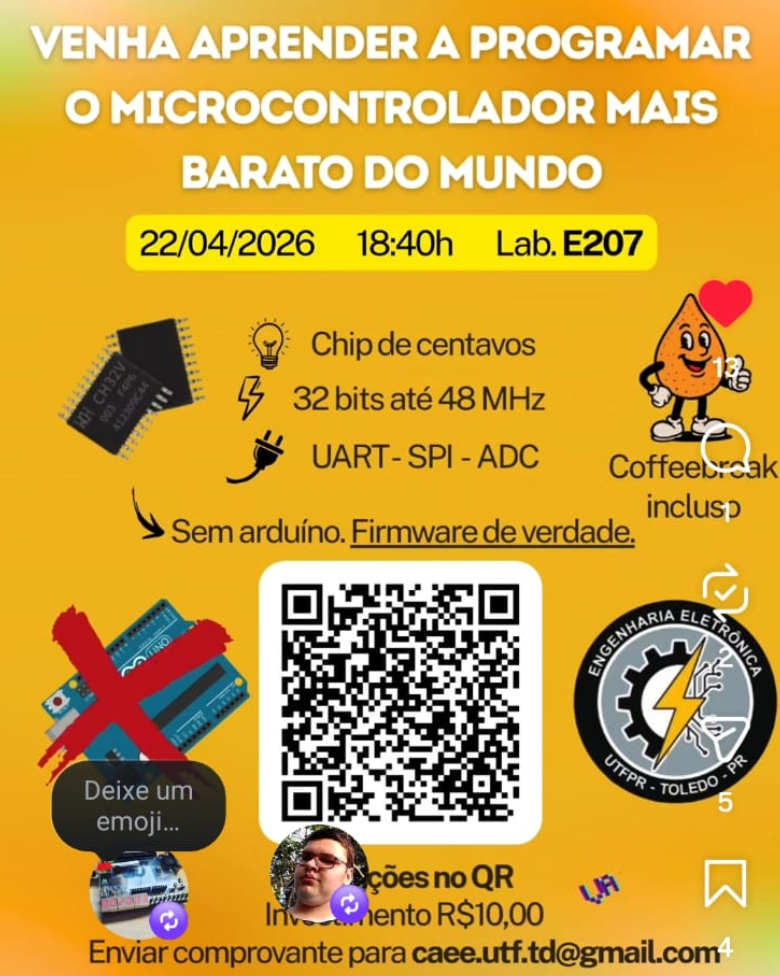
\includegraphics[width=0.56\textwidth]{figuras/image.png}
    \caption{Material de divulgação do minicurso.}
\end{figure}

\clearpage

\begin{figure}[H]
    \centering
    \begin{subfigure}{0.48\textwidth}
        \centering
        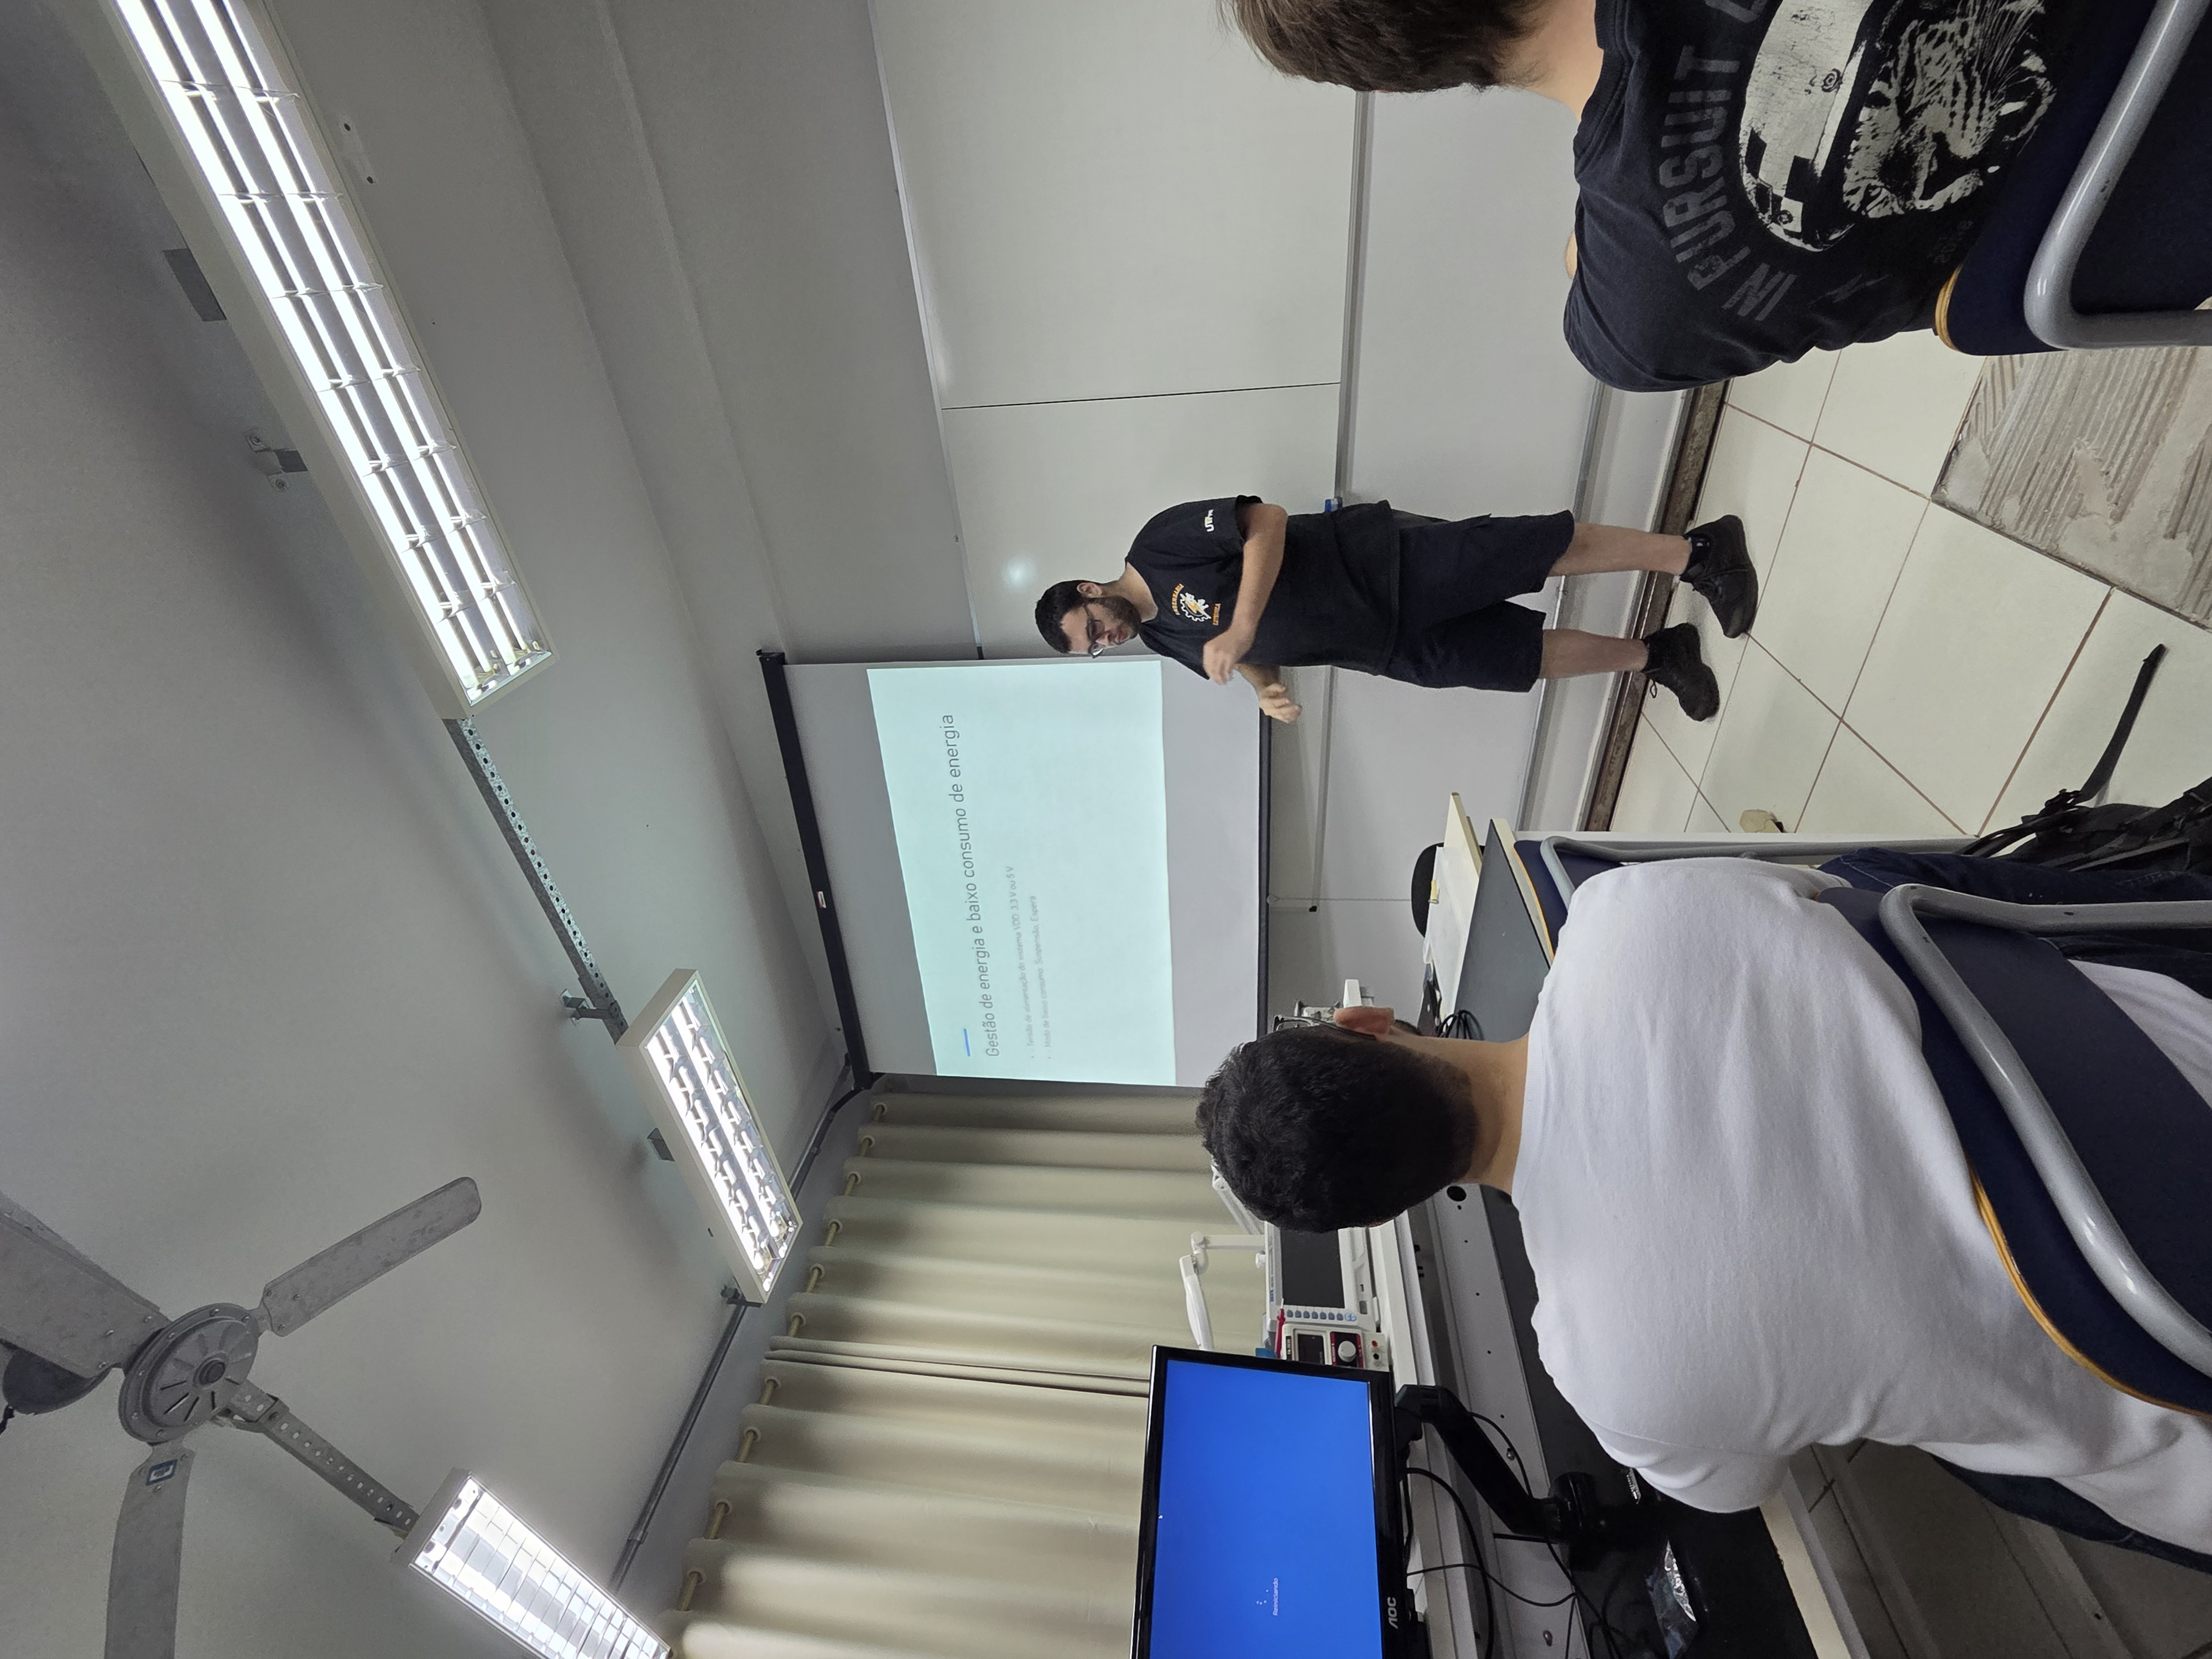
\includegraphics[width=\linewidth,angle=270]{figuras/20260422_185030.jpg}
        \caption{Apresentação inicial da atividade.}
    \end{subfigure}
    \hfill
    \begin{subfigure}{0.48\textwidth}
        \centering
        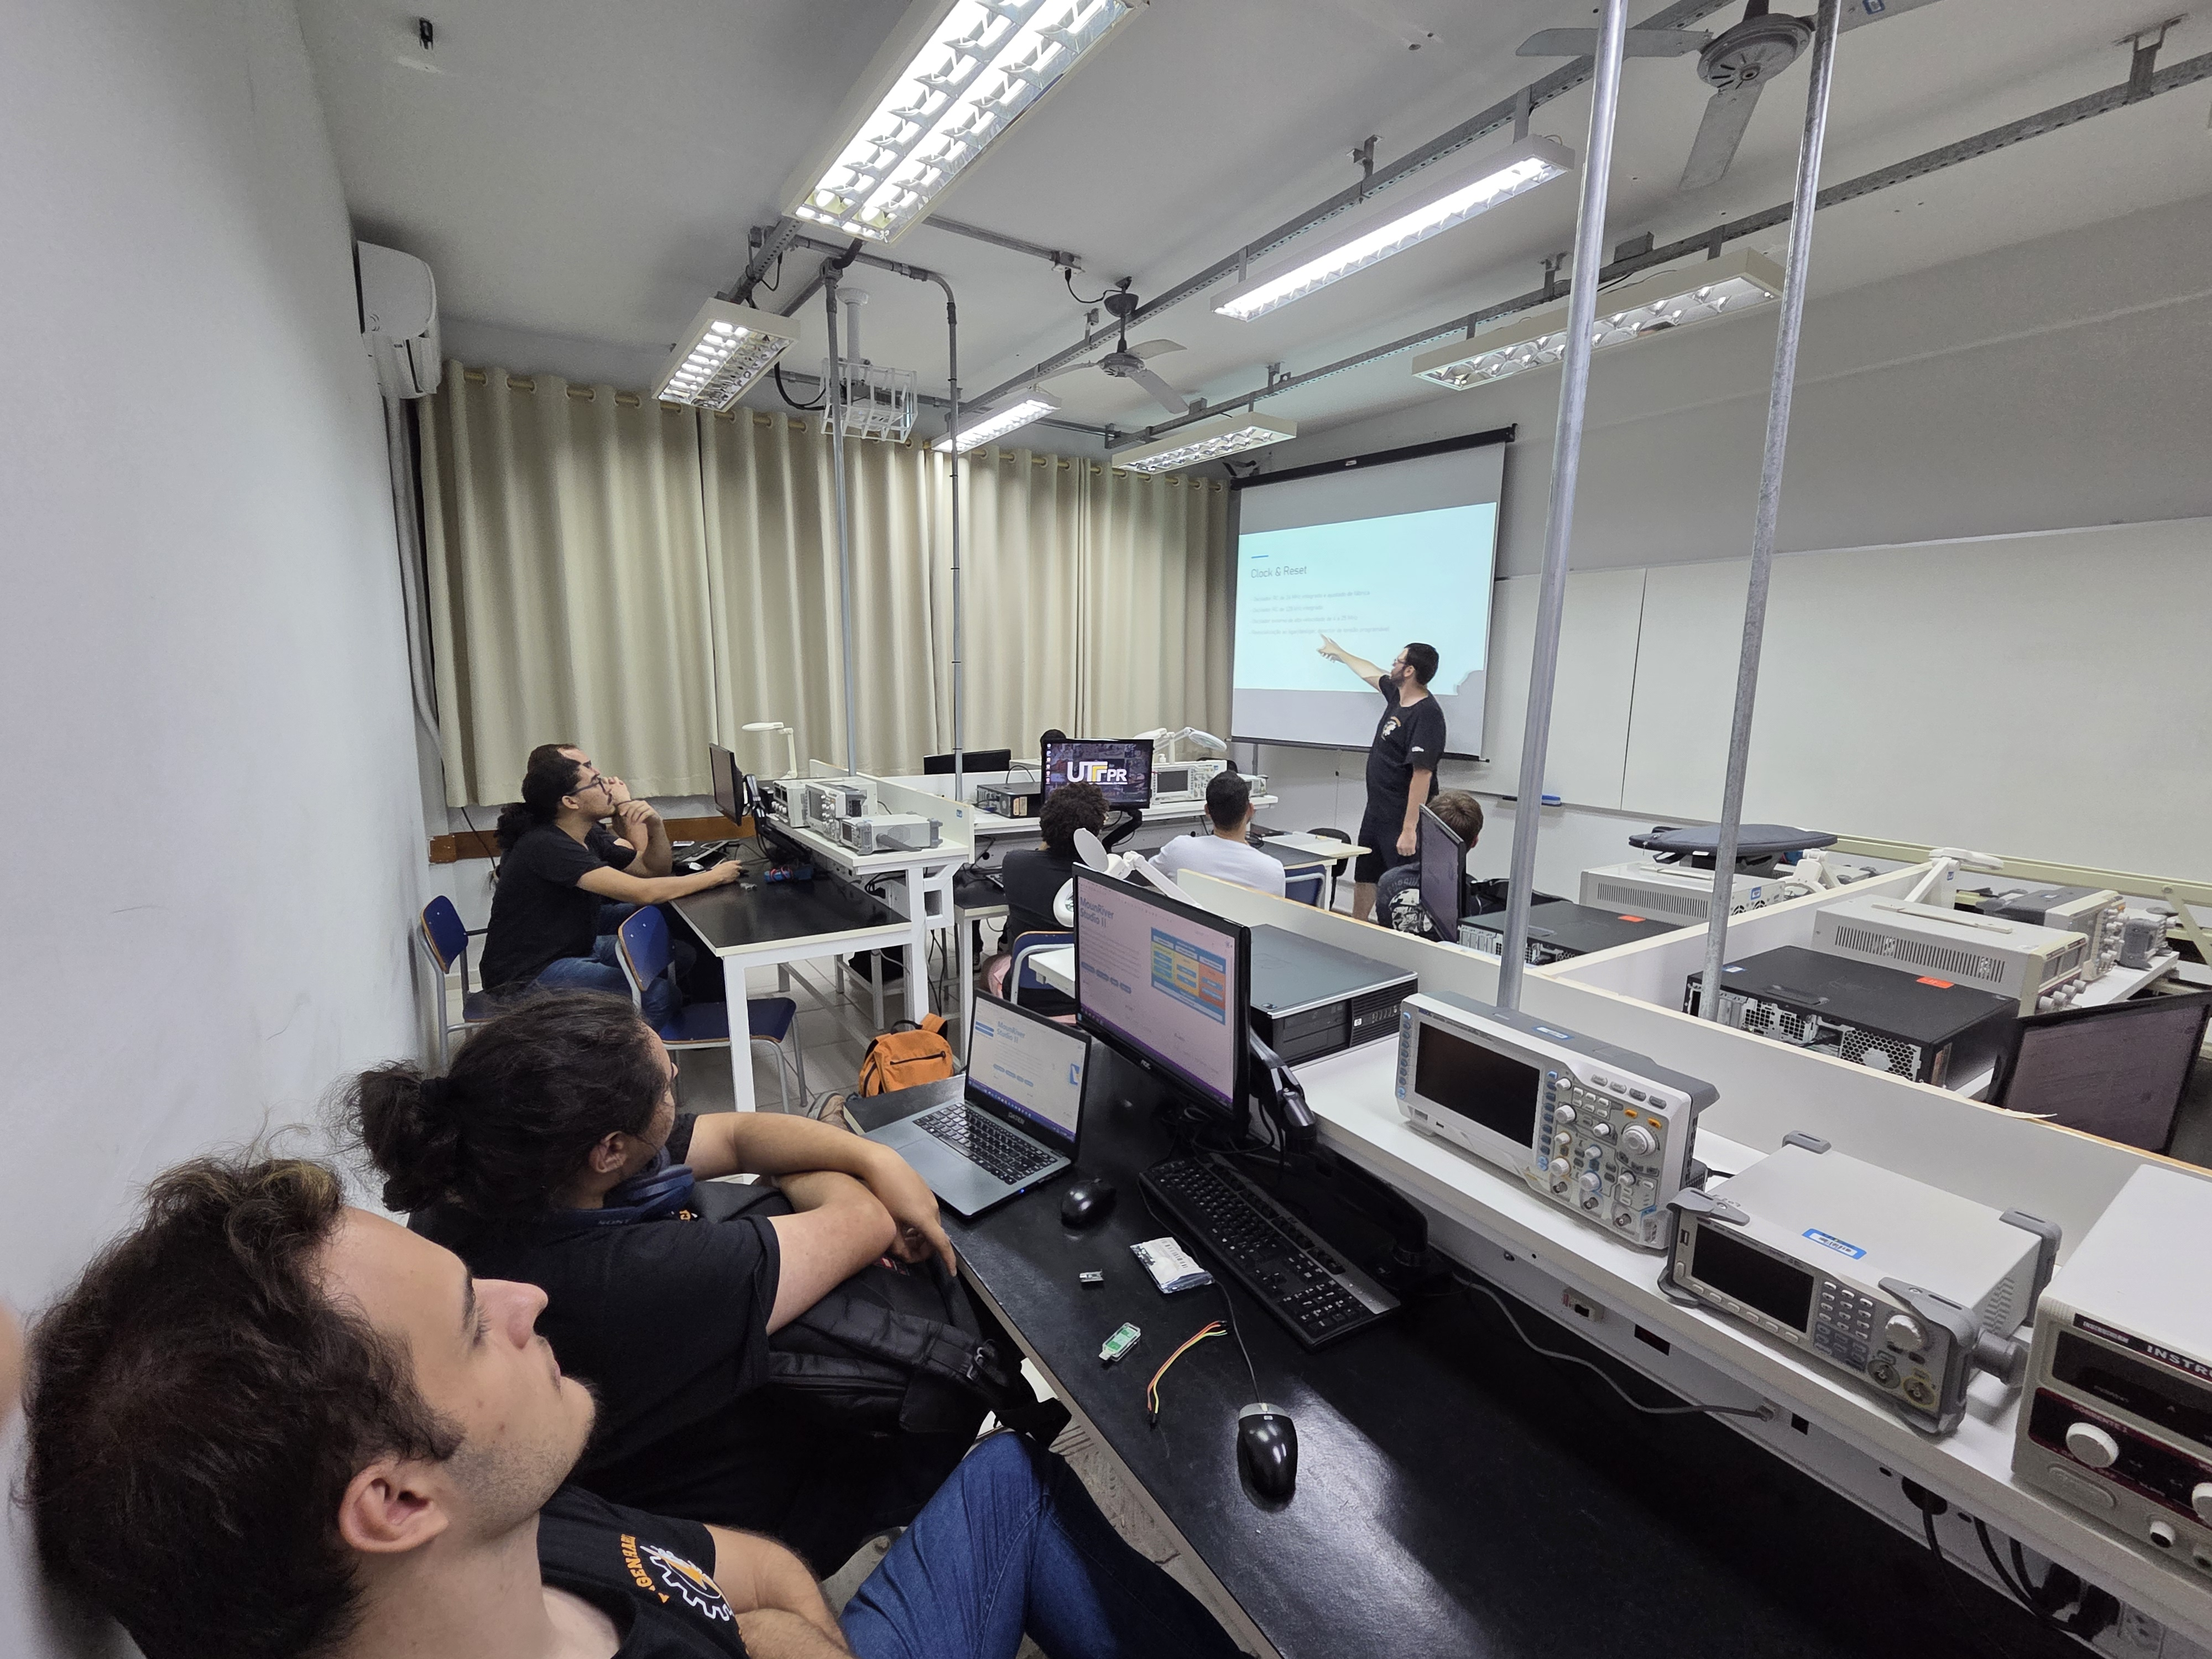
\includegraphics[width=\linewidth,angle=0]{figuras/20260422_185032.jpg}
        \caption{Participantes acompanhando a exposição.}
    \end{subfigure}
    \caption{Exposição inicial do minicurso no Laboratório E207.}
\end{figure}

\begin{figure}[H]
    \centering
    \begin{subfigure}{0.48\textwidth}
        \centering
        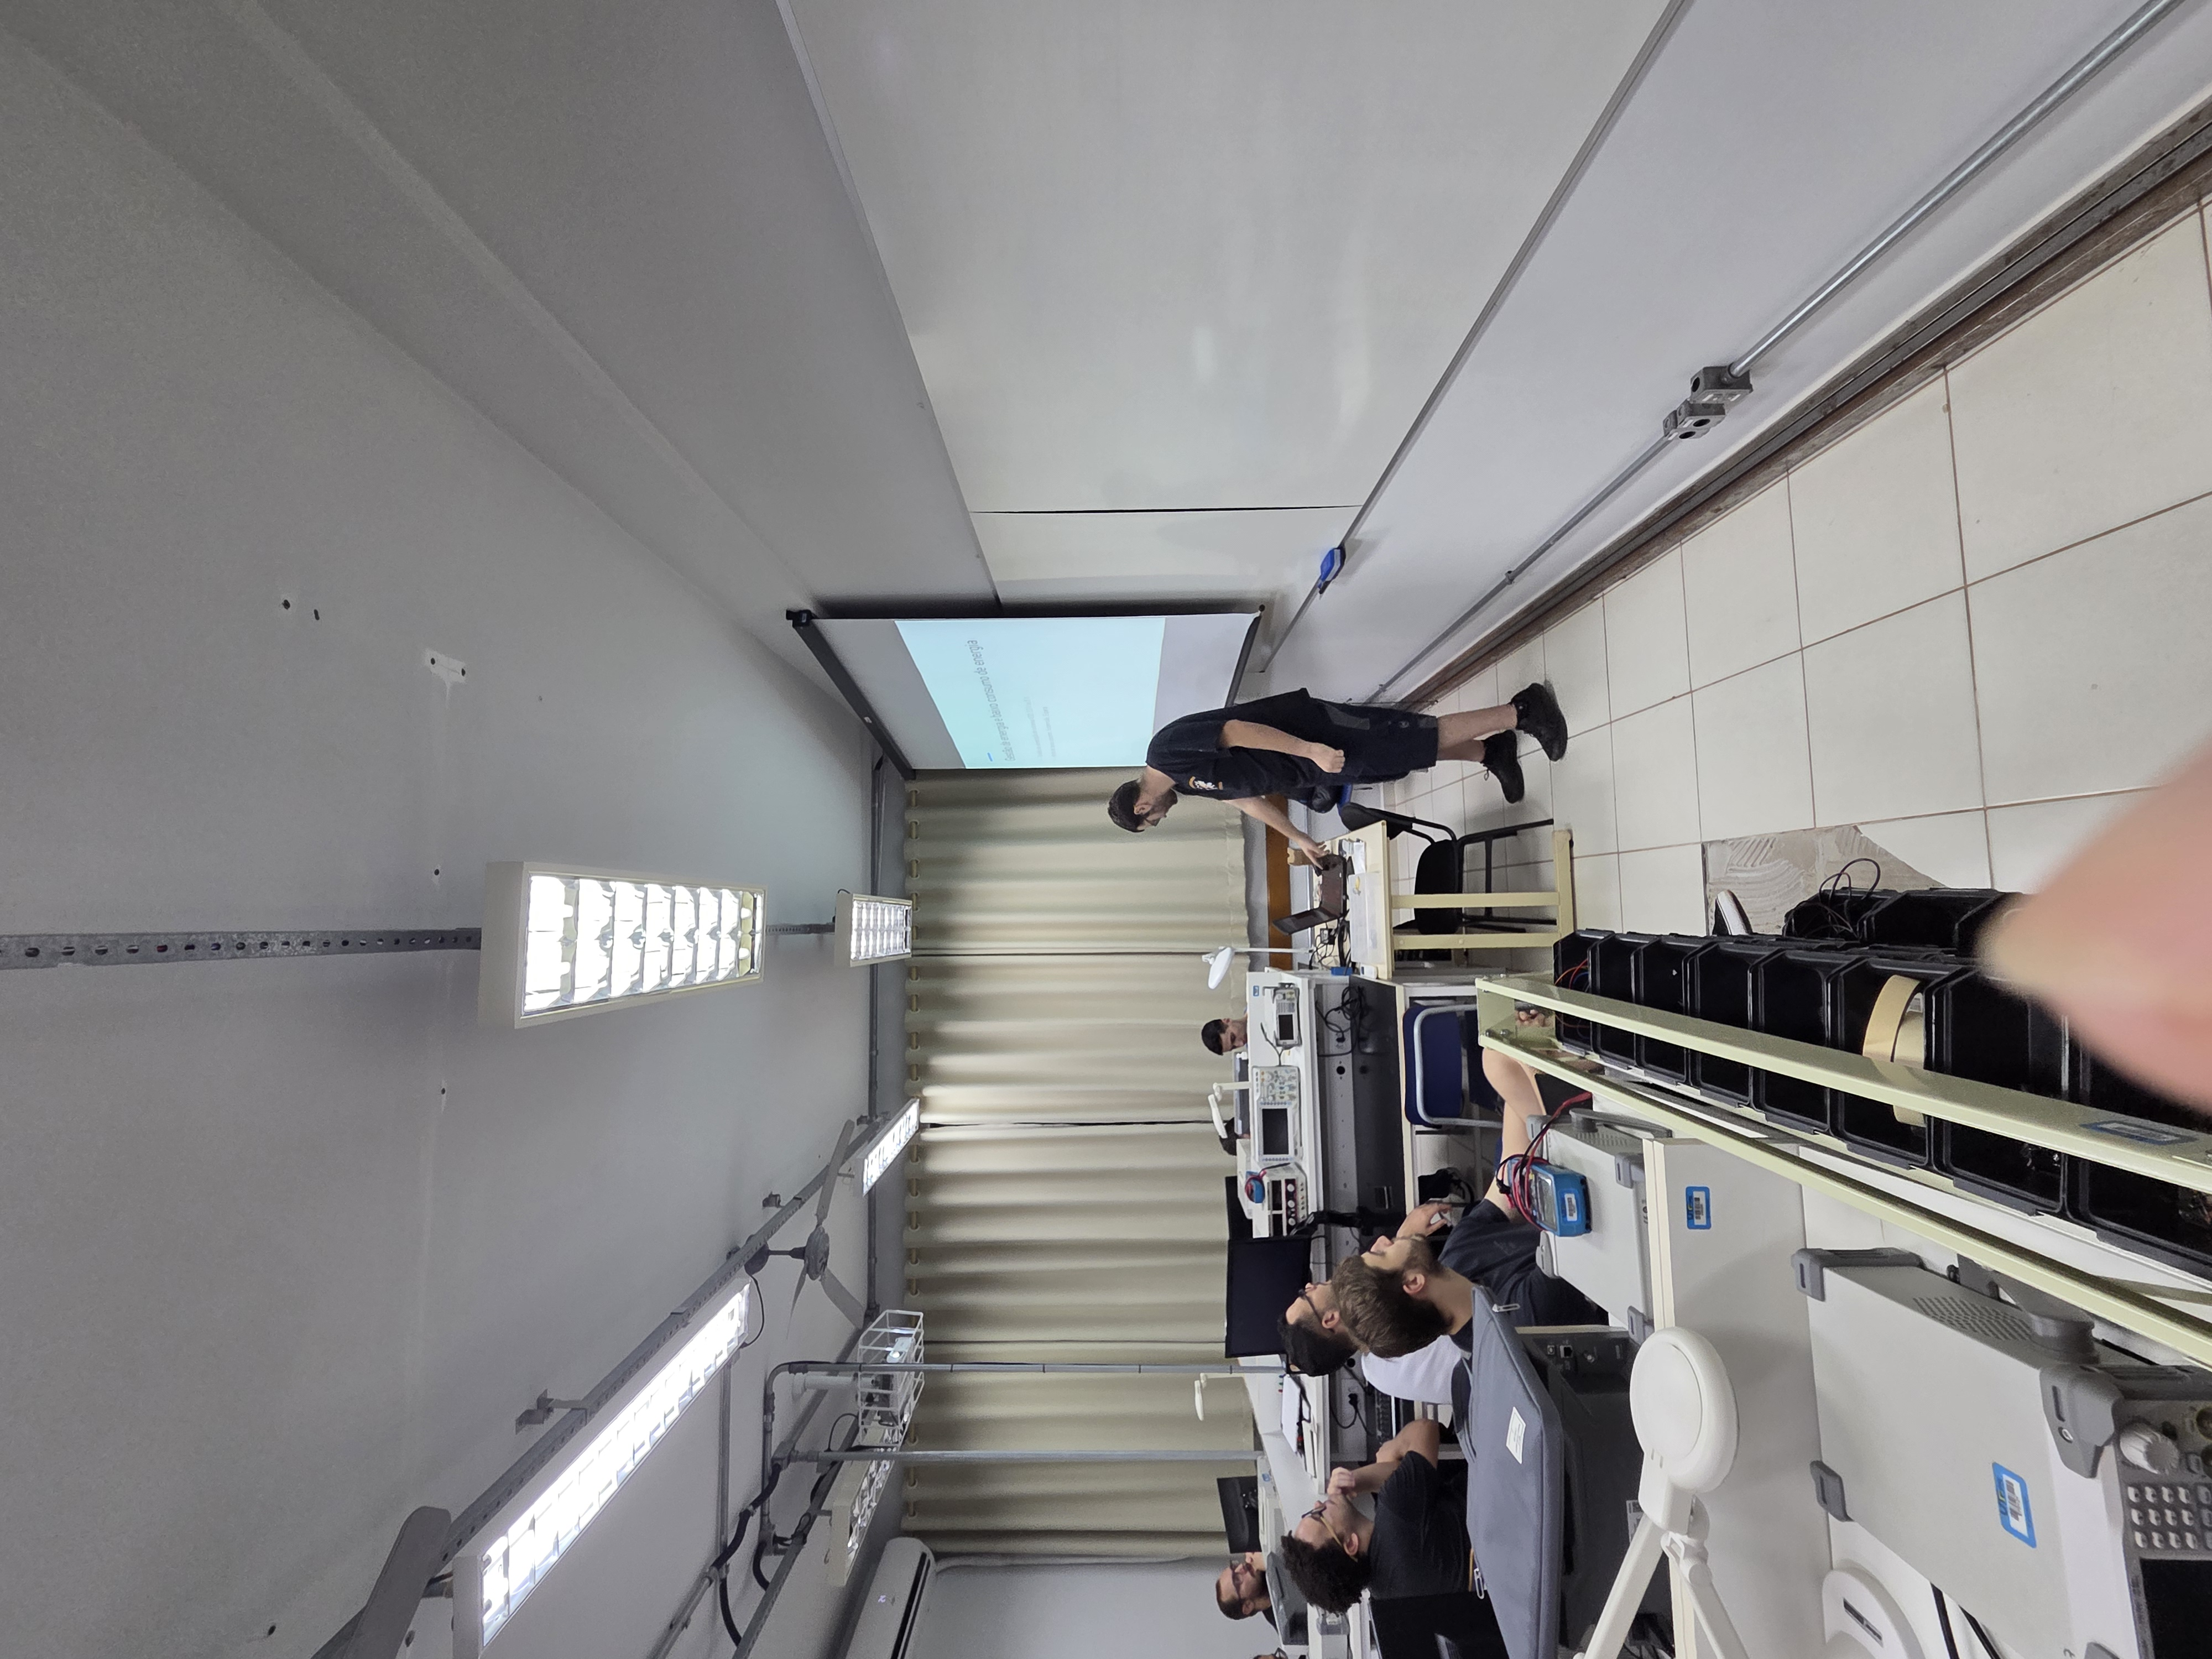
\includegraphics[width=\linewidth,angle=270]{figuras/20260422_185110.jpg}
        \caption{Discussão de conceitos de microcontroladores.}
    \end{subfigure}
    \hfill
    \begin{subfigure}{0.48\textwidth}
        \centering
        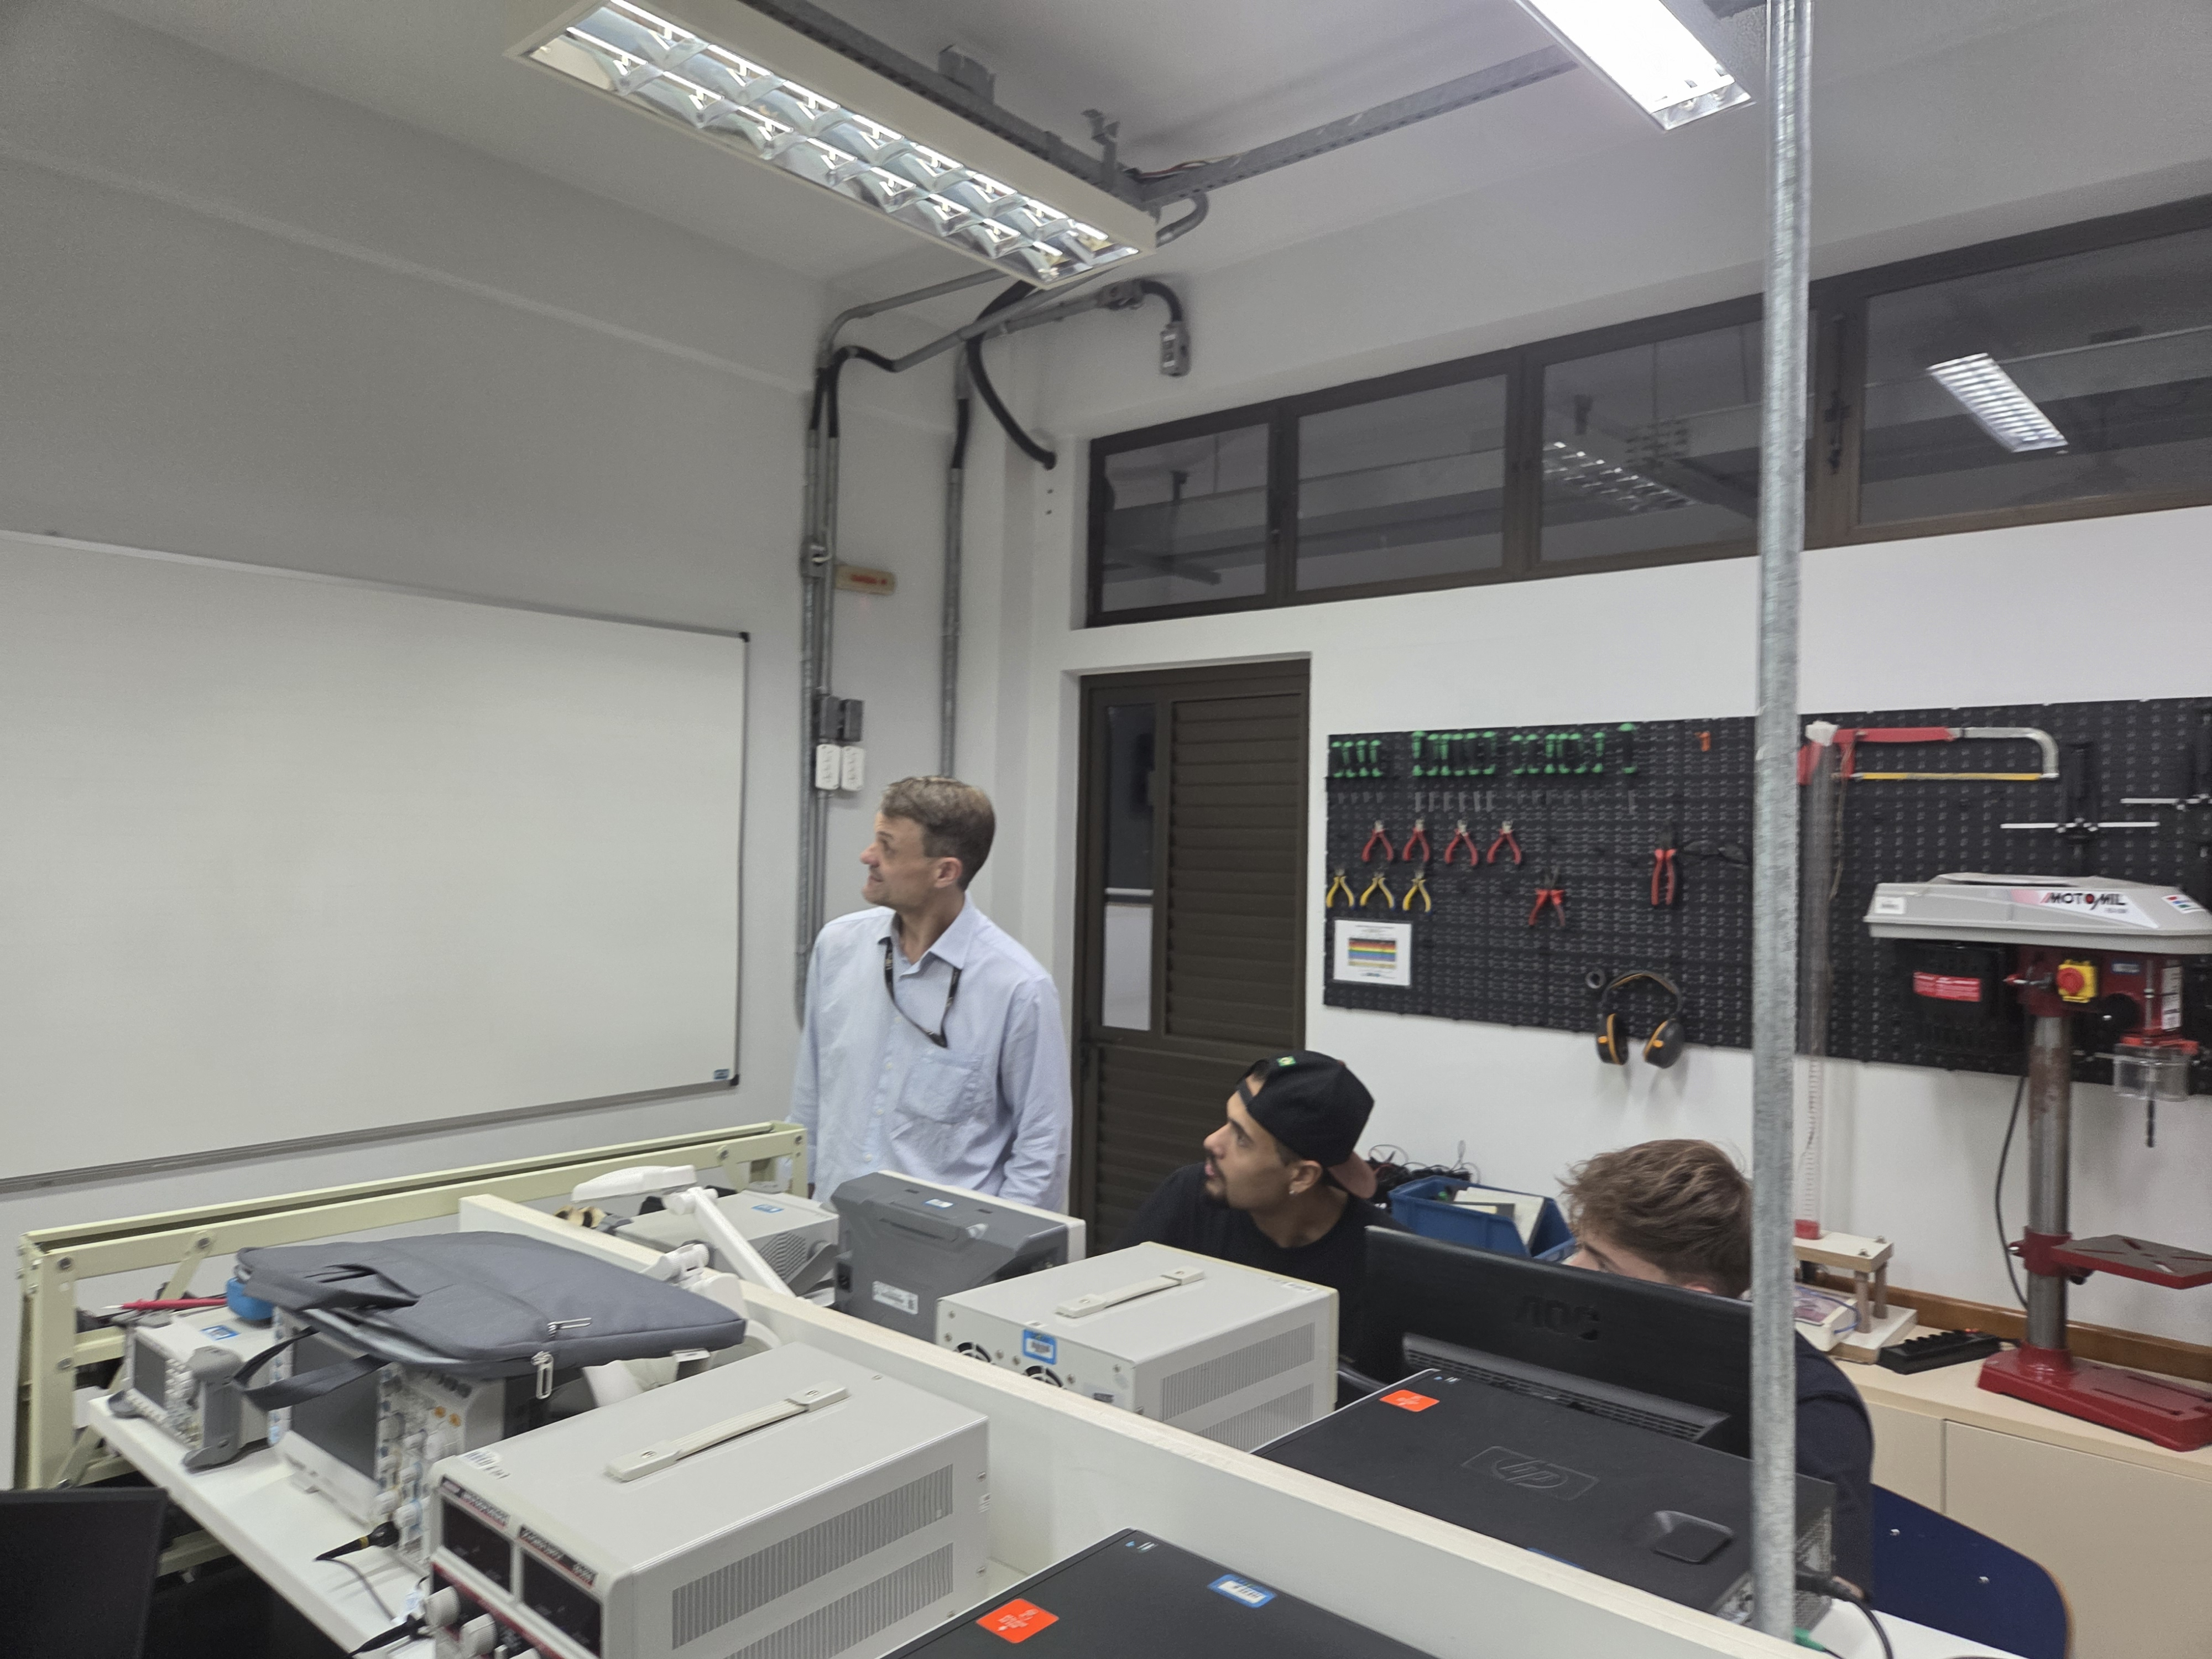
\includegraphics[width=\linewidth]{figuras/20260422_191931.jpg}
        \caption{Atividade em ambiente de laboratório.}
    \end{subfigure}
    \caption{Discussão técnica e interação com os participantes durante o minicurso.}
\end{figure}

\begin{figure}[H]
    \centering
    \begin{subfigure}{0.48\textwidth}
        \centering
        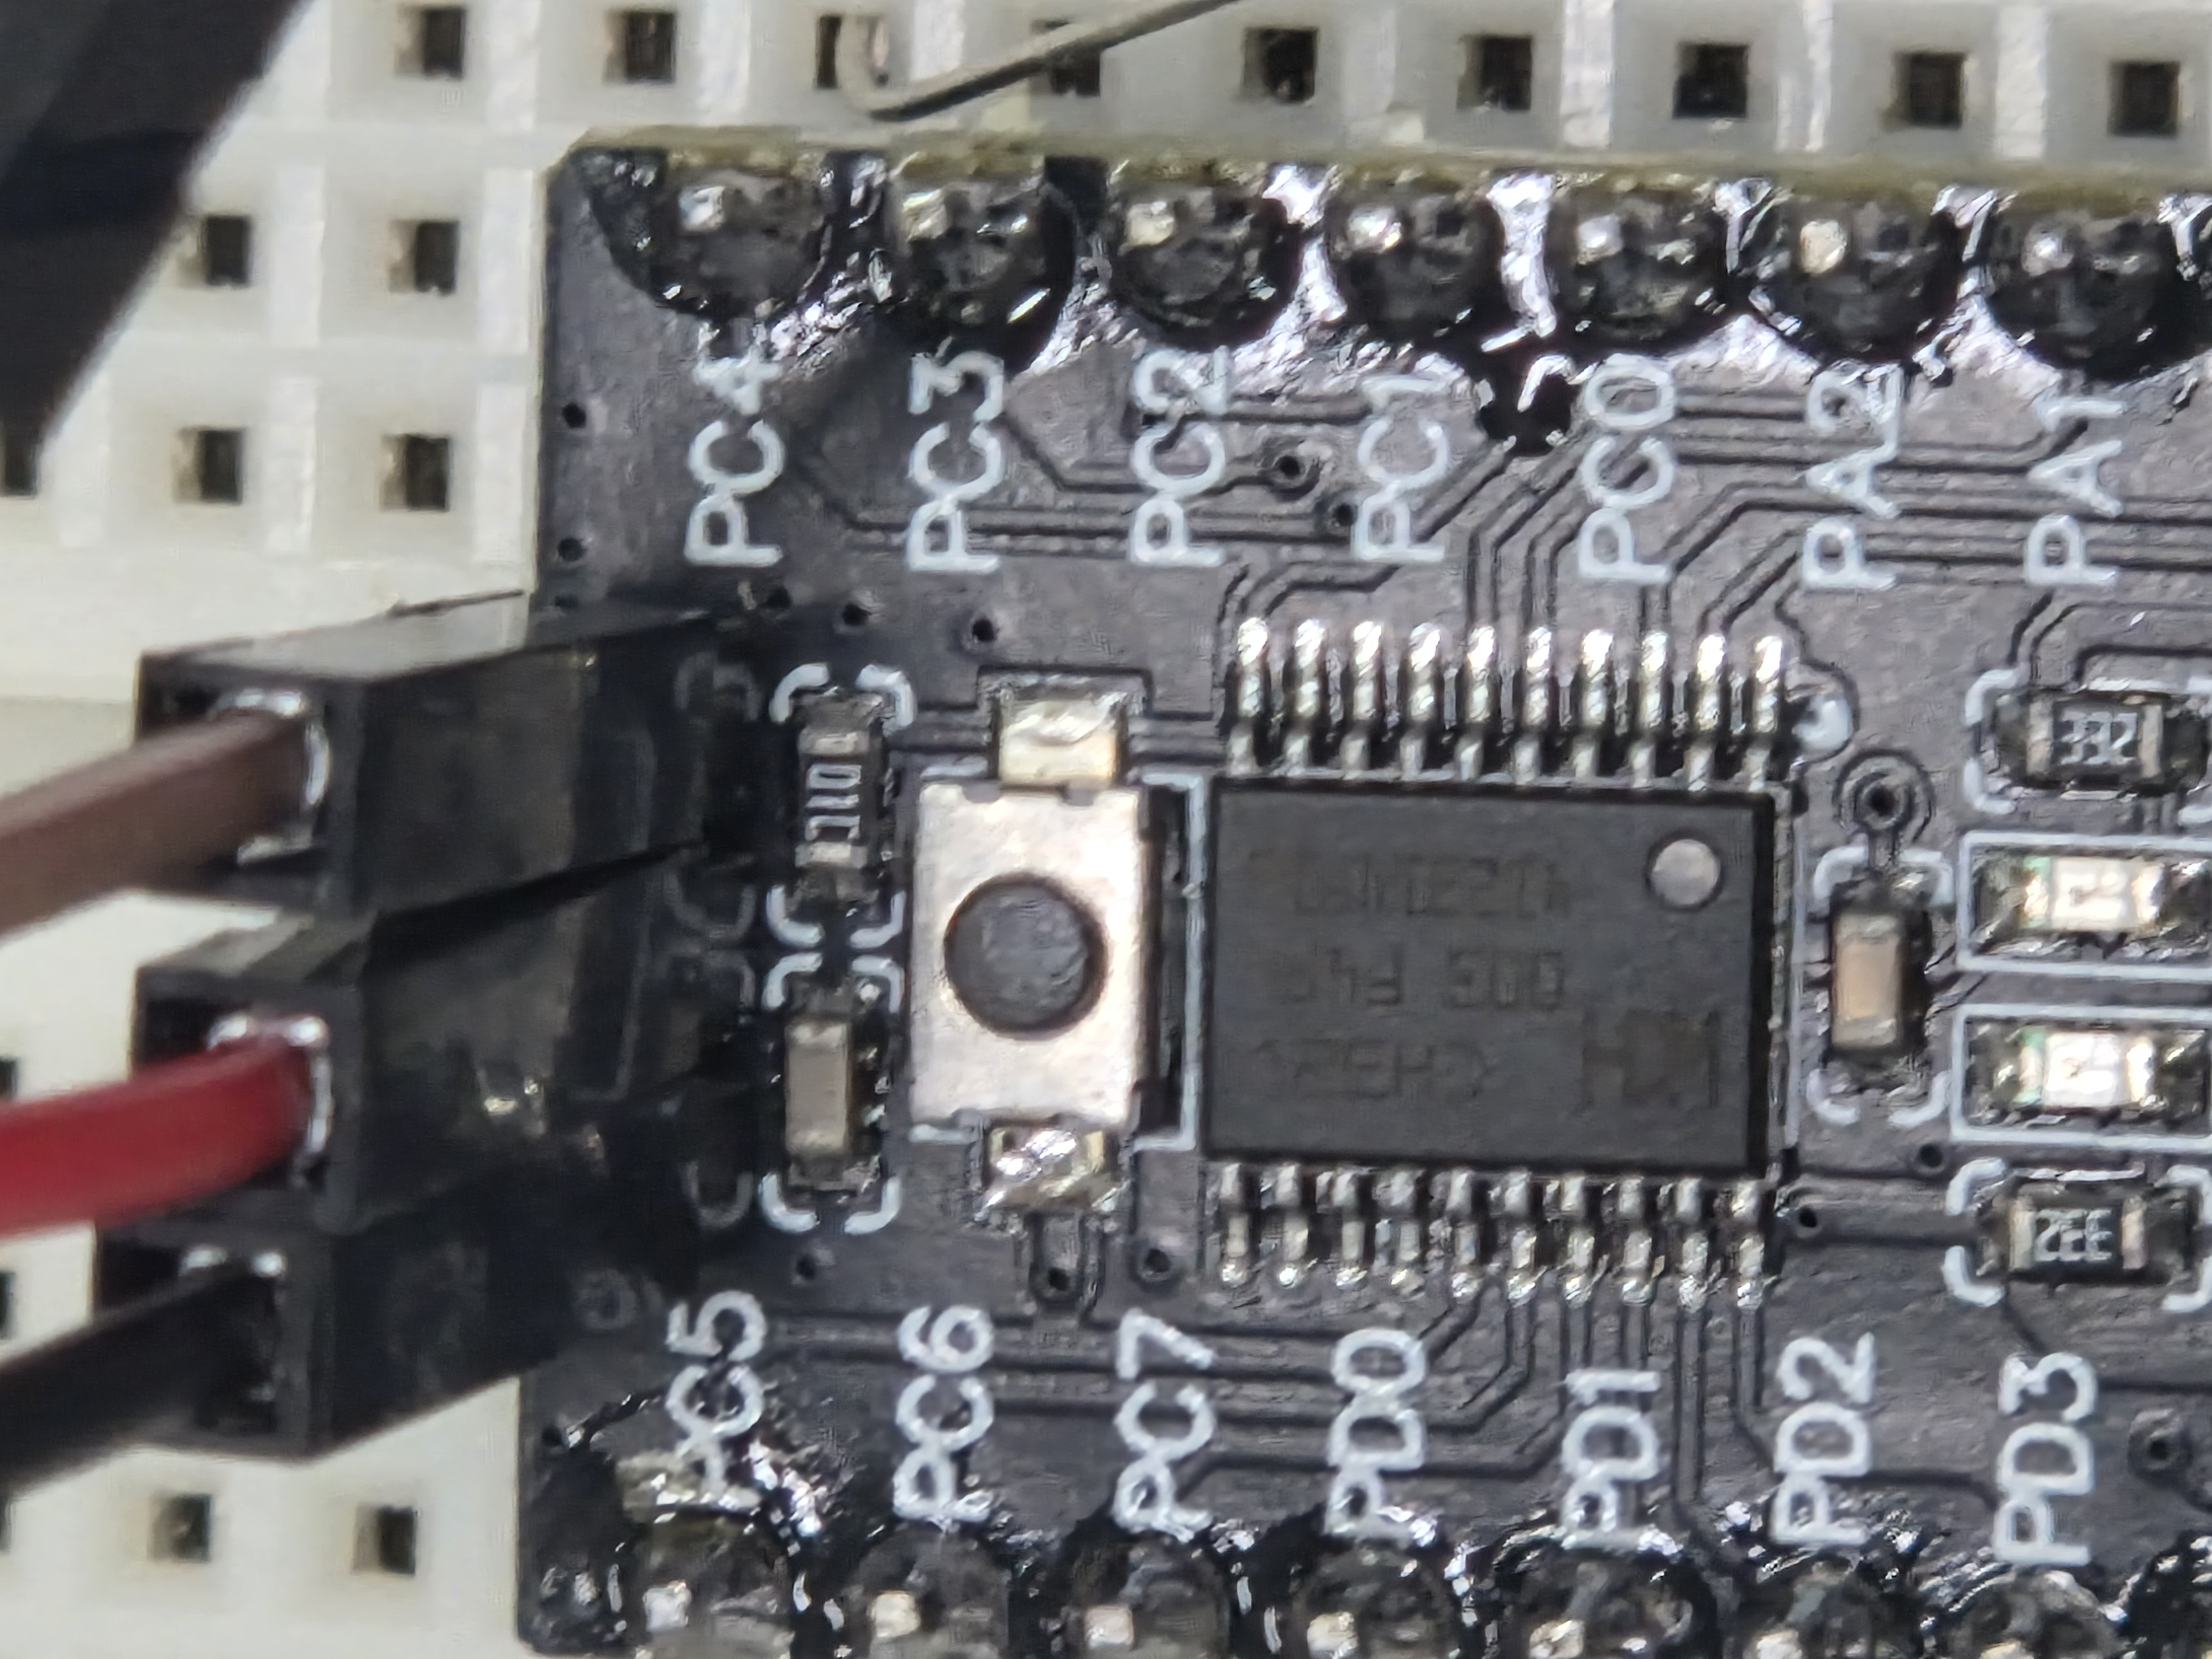
\includegraphics[width=\linewidth]{figuras/20260422_193645.jpg}
        \caption{Microcontrolador CH32V003 em placa de desenvolvimento utilizada na atividade.}
    \end{subfigure}
    \hfill
    \begin{subfigure}{0.48\textwidth}
        \centering
        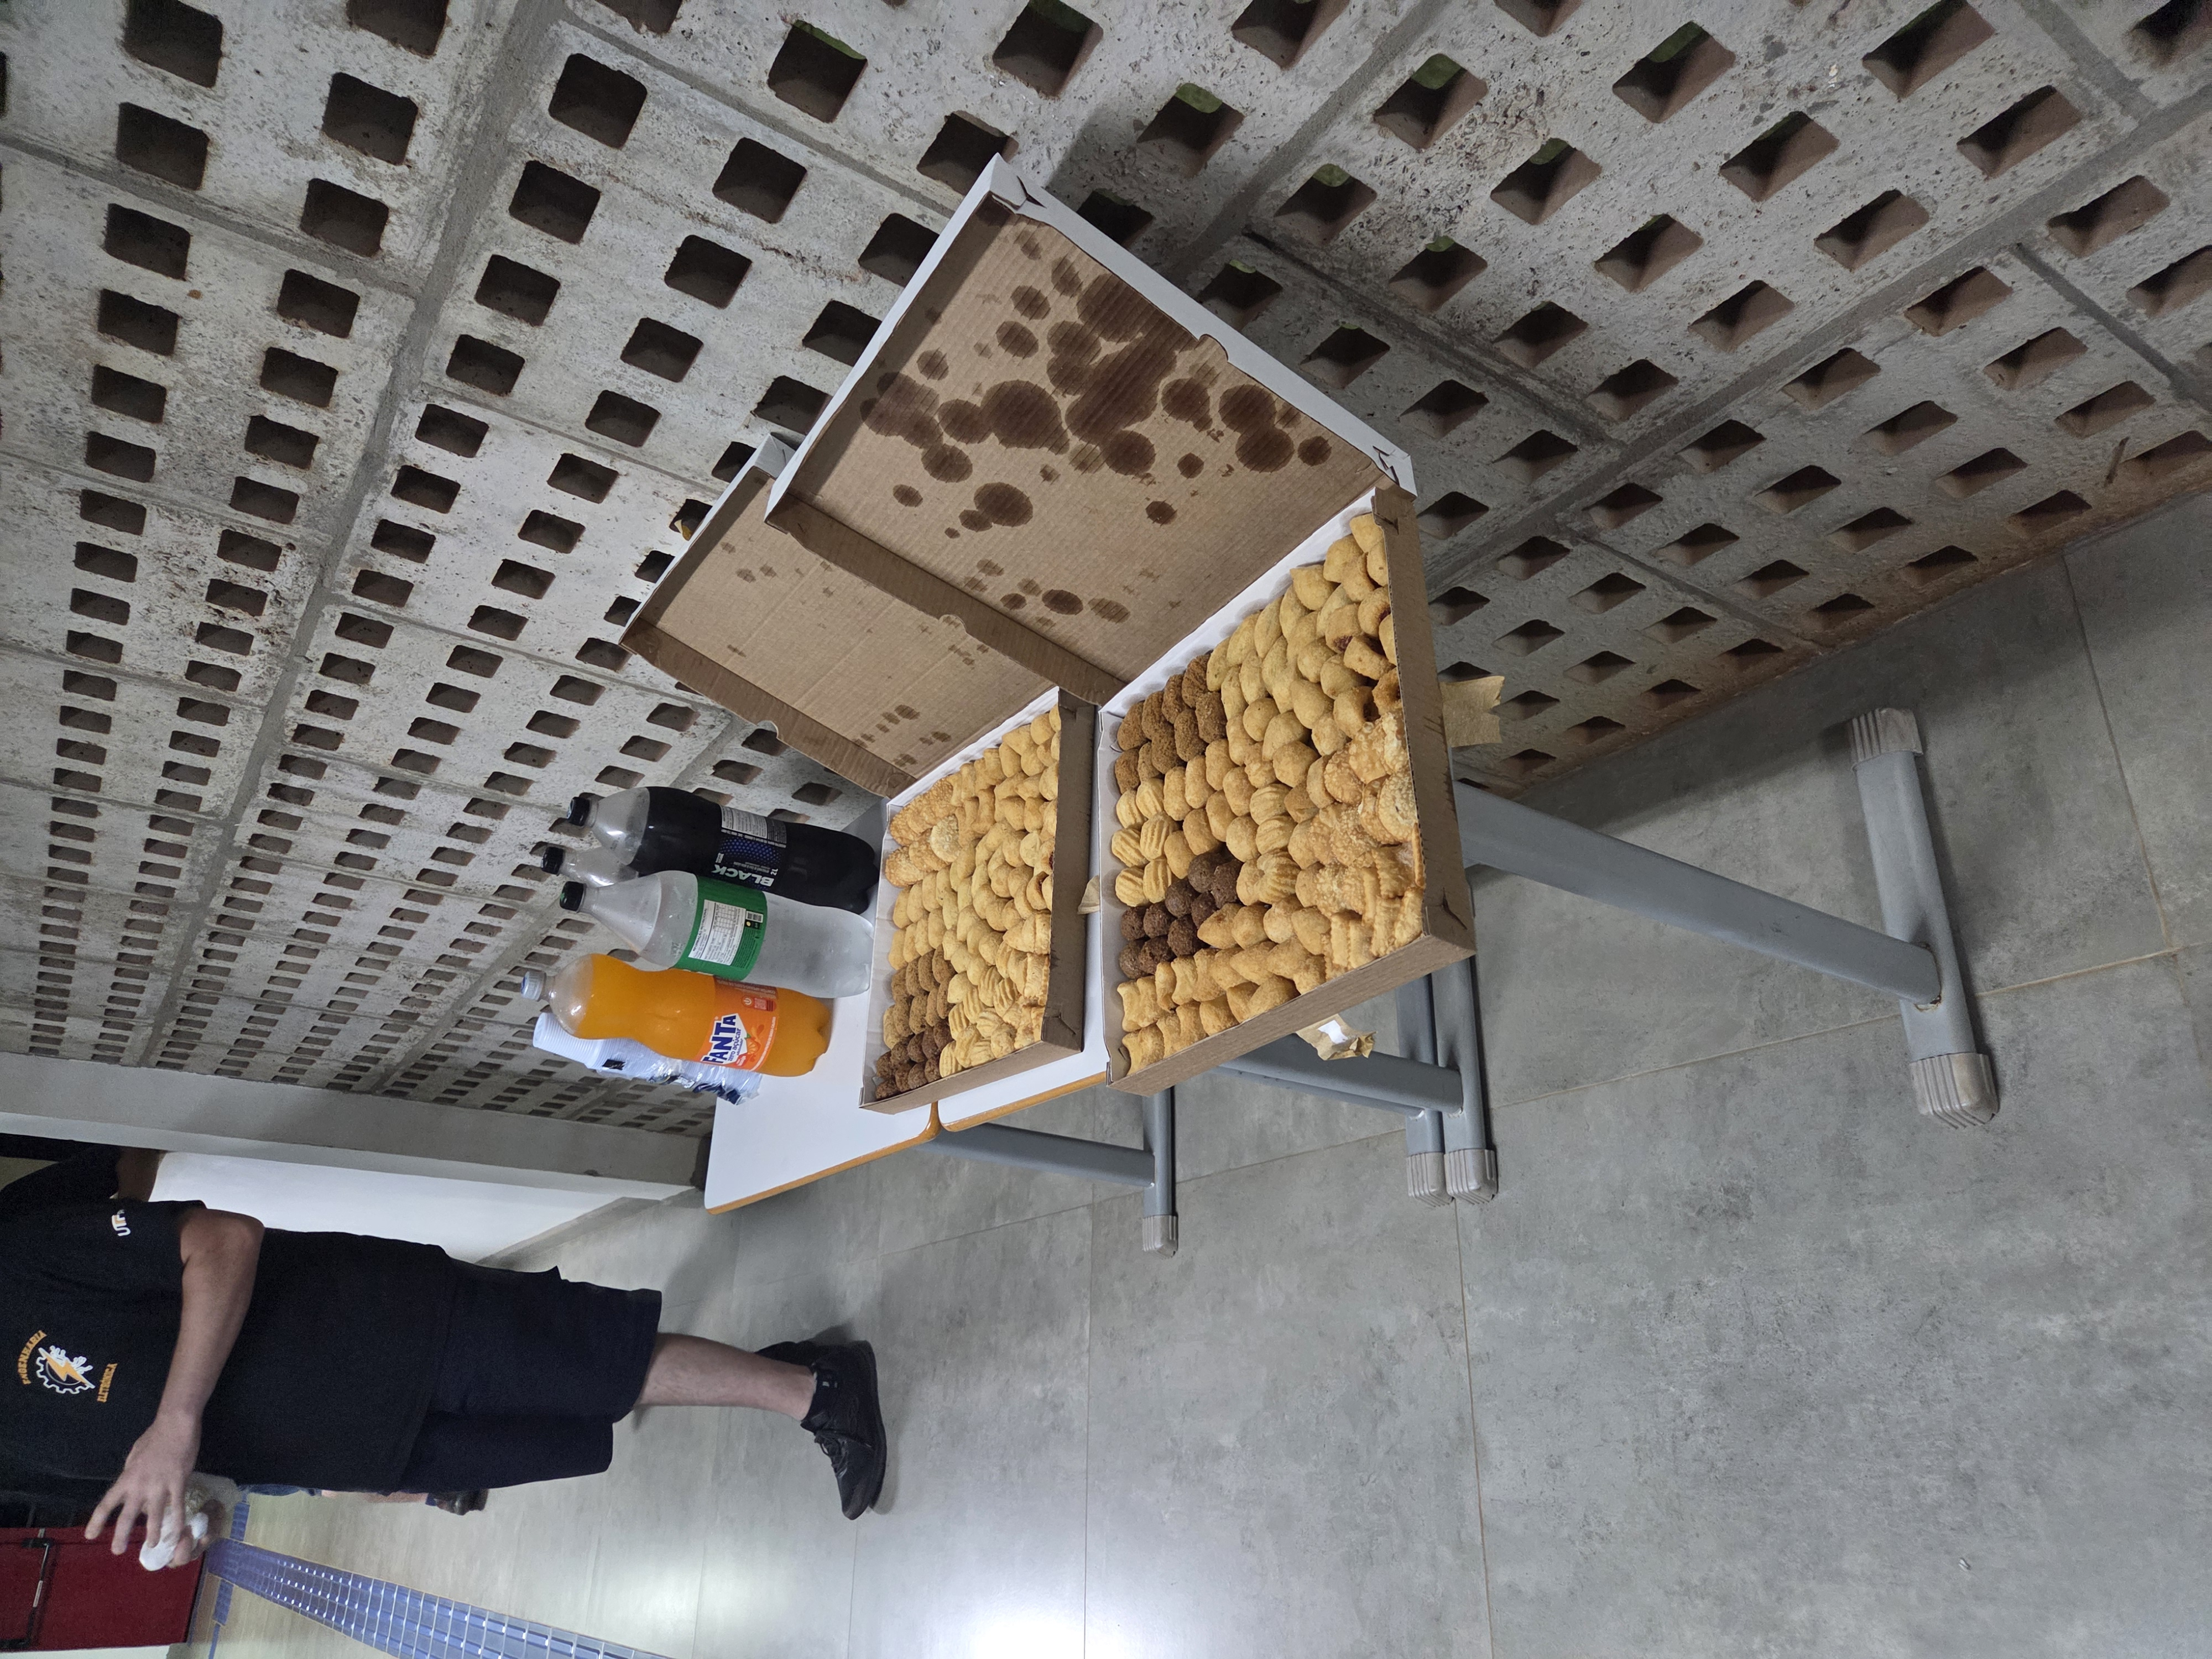
\includegraphics[width=\linewidth,angle=270]{figuras/20260422_204418.jpg}
        \caption{Coffee break ao final do minicurso.}
    \end{subfigure}
    \caption{Registro da placa utilizada no minicurso e momento de encerramento da atividade.}
\end{figure}

\section{Lista de Participantes}

A lista de participantes foi consolidada a partir da relação de inscritos/presença e das listas de alunos regulares dos cursos de Engenharia Eletrônica e Engenharia de Computação. Como alguns registros originais estavam incompletos, os nomes, códigos RA e e-mails foram conferidos por cruzamento entre os documentos disponíveis.

\begin{table}[H]
    \centering
    \small
    \begin{tabularx}{\textwidth}{>{\raggedright\arraybackslash}p{0.38\textwidth}>{\centering\arraybackslash}p{0.16\textwidth}Y}
        \toprule
        \textbf{Nome completo do participante} & \textbf{Código RA} & \textbf{E-mail} \\
        \midrule
        André Hoffmann & 2278367 & \email{ahoffmann@alunos.utfpr.edu.br} \\
        Augusto Aragão Silva & 2461030 & \email{augsl@alunos.utfpr.edu.br} \\
        Enzo Paiva Ramos & 2314606 & \email{enzopaiva@alunos.utfpr.edu.br} \\
        Gabriel Angeli de Almeida & 2370883 & \email{gabrielangeli@alunos.utfpr.edu.br} \\
        Gabriel Mateus Cavalheiro & 2035545 & \email{cavalheiro@alunos.utfpr.edu.br} \\
        Guilherme Alexandre Livi Chini & 2369427 & \email{guilhermechini@alunos.utfpr.edu.br} \\
        Luccas Hernanny Lima Johann & 2460556 & \email{luccasjohann@alunos.utfpr.edu.br} \\
        Luís Vinícius Balta Nunes & 2614421 & \email{luisvinicius@alunos.utfpr.edu.br} \\
        Marco Antônio Amaral Galante & 2205068 & \email{marcoantoniogalante@alunos.utfpr.edu.br} \\
        Pietro Rodrigues Kalinoski & 2777851 & \email{pietrokalinoski@alunos.utfpr.edu.br} \\
        Samuel Eudes Heinrichs & 2295733 & \email{samuelheinrichs@alunos.utfpr.edu.br} \\
        Vinícius Eduardo Ganda de Carvalho & 2871084 & \email{vinicius.e.g.carvalho@gmail.com} \\
        \bottomrule
    \end{tabularx}
    \caption{Participantes identificados no minicurso.}
\end{table}

\section{Outras Informações}

O material de divulgação informa que o minicurso teve como chamada principal ``Venha aprender a programar o microcontrolador mais barato do mundo'', destacando características como chip de baixo custo, arquitetura de 32 bits com operação até 48 MHz e periféricos UART, SPI e ADC. Também foi indicado que a atividade abordaria firmware em baixo nível, sem uso da plataforma Arduino, e que haveria coffee break incluso.

Foram disponibilizados registros em vídeo da atividade na pasta de figuras original do projeto. Os vídeos não foram incorporados ao presente relatório em PDF, mas permanecem como documentação complementar da execução da ação.

\end{document}
